\chapter[Open issues in resource-constrained JVMs]{Open issues in \\ resource-constrained JVMs}

\begin{table}
\caption{Point requiring attention in future sensor node VMs}
\label{tbl-issues}
    \centerline{
    \begin{tabular}{llll} % NO SIMULATION DATA
    \toprule
    Section                     &  Issue                                        &  in                   &  affects          \\
    \midrule
    \midrule
    \ref{sec-std-lib}           & A tailored standard library                   & Standard library      & VM size \\
    \ref{sec-const-data}        & Support for constant arrays                   & Source language, VM   & memory usage, code size \\
    \ref{sec-nested-data}       & Support for nested data structures            & Source language, VM   & memory usage, performance \\
    % \ref{sec-small-datatypes}   & Better lang. support for shorts and bytes     & Source language       & memory usage, source maintainability \\
    \ref{sec-small-datatypes}   & Better lang. support for shorts and bytes     & Source language       & memory usage, \\
                                &                                               &                       & ~~  source maintainability\\
    \ref{sec-typedef}           & Simple type definitions                       & Source language       & source maintainability \\
    \ref{sec-inlining}          & Explicit and efficient inlining               & Source language       & performance \\
    \ref{sec-optimising-javac}  & An optimising compiler                        & Compiler              & performance \\
    \ref{sec-no-gc}             & Allocating objects on stack                   & Source language, VM   & (predictable) performance \\
    \ref{sec-advanced-features} & Reconsidering adv. language features          & Source language, VM   & VM size, complexity, \\
                                & ~~threads, exceptions, OO, garbage collection &                       & ~~ and performance \\
    \bottomrule
    \end{tabular}
    }
\end{table}


\label{sec-lessons-from-jvm}

In Section \ref{sec-introduction-research-questions} we defined two of our main research questions as how close an AOT compiling sensor node VM can come to native performance, and whether a VM is an efficient way to provide a safe execution environment. These questions are not specific to Java, and the main motivation to base CapeVM on Java was the availability of a rich set of tools and infrastructure to build on, including a solid VM to start from in the form of Darjeeling. In this chapter we consider the third question: whether Java is a suitable language for a sensor node VM, and how it may be improved.

One aspect of the JVM that makes it an attractive choice for sensor nodes is its simplicity, allowing a useful subset of it to be implemented in as little as 8 KB \cite{Harbaum}. However, it also lacks some important features which ultimately makes it a less good fit for typical sensor node code. These range from minor annoyances that reduce code readability, to the lack of support for constant data and high memory consumption for nested data structures. The last two issues make some applications that can run on a sensor node when written in C, impossible to implement in standard Java.

In this chapter we discuss the most pressing issues we encountered, summarised in Table \ref{tbl-issues}, and suggest ways they could be improved in future VMs. Where possible, the impact of these issues is quantified in Table \ref{tbl-quantitative-results}. Although more study is required to turn these suggestions into working solutions, many of the points raised here could be improved with minor changes to Java, leading to a 'sensor node Java', much like nesC \cite{Gay:2003up} is a sensor node version of C, but some require more drastic changes.




\section{A tailored standard library}
\label{sec-std-lib}

A minimum Java API for resource-constrained devices, the Connected Limited Device Configuration (CLDC) specification, was proposed by Sun Microsystems \cite{CLDC}. The CLDC was primarily intended for devices larger than typical sensor nodes, and not tailored to the characteristics of typical sensor node code. Providing support for the full CLDC specification would require a substantial amount of memory and programme space for features that are rarely required by sensor node applications. Table \ref{tab-vm-size} shows the code size of library support as implemented in the original Darjeeling VM.

The largest mismatch comes from the CLDC's string support, which takes up over 10 KB. While string support is one of the most basic features one would expect to find in the standard library of any general purpose language, it is rarely required within sensor node applications that usually do not have a UI and only communicate with the outside world through radio messages.

On the other hand, the standard library should include abstractions for typical sensor node operations that are missing from the CLDC. The CLDC \mycode{Stream} abstraction is intended to facilitate file, network and memory operations. The abstraction is not well suited for communication protocols required by sensor node applications, such as I$^{2}$C and SPI. In CLDC, connections between devices can be initiated by specifying URI-like strings. However, processing these is relatively expensive, and sensor nodes often identify each other using a 16 or 32-bit identifier.

\begin{table}
\caption{Size of Darjeeling VM components}
\label{tab-vm-size}
    \begin{tabular}{lrrcr} % NO SIMULATION DATA
    \toprule
    Component             & std.lib                   & VM                   & & total \\
                          & (bytes)                   & (bytes)              & & (bytes)  \\
    \midrule
    \midrule
    Core vm               &  3529                     &  7006                & &           10535 \\
    Strings               &  8467                     &  1942                & &           10409 \\
    Interpreter loop      &     0                     & 10370                & &           10370 \\
    Garbage collection    &    80                     &  3442                & &            3522 \\
    Threads               &   909                     &  2472                & &            3381 \\
    Exceptions            &  1338                     &   818                & &            2156 \\
    Math                  &   222                     &  1274                & &            1496 \\
    IO                    &   530                     &   680                & &            1210 \\
    Total                 & 15075                     & 28004                & &           43079 \\
    \bottomrule
    \end{tabular}
\end{table}
 

Aslam \cite{Aslam:2011thesis} discusses a method for dead code removal that could be used to remove unused code from a library. The remaining library code becomes part of the application that is uploaded to a device as a whole. While this can be useful to allow developers to use a large library of seldom used functions that will only be included when needed, this is much less efficient compared to a natively implemented standard library, and not possible for library functions to access the hardware.

Therefore we argue a minimal tailored library is necessary that may be efficiently implemented in native code and present on all devices, and that this library should be designed from the ground-up specifically for sensor node applications. Such a library should include functionality for: (i) basic math; (ii) array operations; (iii) a communication API that encapsulates the low-level protocols typically used (e.g. I$^{2}$C); and (iv) a higher-level generic radio and sensor API abstraction.


\clearpage
\newgeometry{margin=1cm}
\thispagestyle{empty}
\begin{landscape}
\begin{table}[t!]
\caption{Quantitative impact of Java/JVM issues}
\label{tbl-quantitative-results}
    \centerline{
    \begin{threeparttable}
    \begin{tabular}{llrrrrrrrrrrrrrrr} % UPDATED 20180313
    \toprule
    Section                    & Measure \tnote{a}                    &      B.sort &      H.sort &   Bin.Search &       XXTEA &    MD5 &       RC5 &           FFT & Outlier &           LEC &       CoreMark &                MoteTrack & HeatCalib & HeatDetect \\
    \midrule
    \midrule
    \ref{sec-const-data}       & Size of constant data                &             &             &              &             &        &       200 &         2,048 &         &            51 &                &                   20,560 &           &            \\
                               & Const array RAM overhead             &             &             &              &             &        &       208 &  \tblhl 2,056 &         &            67 &                &           \tblhl too big &           &            \\
                               & Const array flash overhead           &             &             &              &             &        &     1,998 & \tblhl 26,714 &         &           930 &                &           \tblhl too big &           &            \\
    \ref{sec-nested-data}      & Size of main data structures in C    &         512 &         512 &          200 &         144 &    174 &       256 &           256 &     860 &          1024 & 1633 \tnote{b} &                      606 &       644 &       1088 \\
                               & Size of main data structures in Java &         520 &         520 &          208 &         160 &    214 &       288 &           272 &     884 &          1058 &           1983 & \tblhl    1387 \tnote{c} &       676 &       1158 \\
                               & Size increase                        &       1.6\% &       1.6\% &        4.0\% &      11.1\% & 23.0\% &    12.5\% &         6.3\% &   2.8\% &         3.3\% &         21.4\% &           \tblhl 128.9\% &     5.0\% &      6.4\% \\
    \ref{sec-small-datatypes}  & Casts                                &           1 &           6 &            5 &           8 &      8 &         8 &            16 &       3 &             8 &             41 &                       33 &         4 &         70 \\
                               & Lines of code \tnote{d}              &          11 &          24 &           16 &          38 &    165 &        27 &            73 &      43 &            48 &            637 &                      475 &        47 &        272 \\
                               & Casts per 100 LOC                    &           9 &   \tblhl 25 &    \tblhl 31 &          21 &      5 & \tblhl 30 &            22 &       7 &            17 &              6 &                        7 &         9 &  \tblhl 26 \\
    \ref{sec-inlining}         & Slowdown non-inlined version         &             & \tblhl 69\% &              & \tblhl 57\% &   25\% &      37\% &          20\% &         &               &            8\% &                          &           &            \\
                               & Size difference non-inlined version  &             &         +42 &              &        -224 &  -1502 &       -94 &           -20 &         &               &            +48 &                          &           &            \\
    \ref{sec-optimising-javac} & Slowdown w/o optimisations           & \tblhl 91\% & \tblhl 52\% & \tblhl 544\% &         3\% &        &           &           3\% &    23\% &               &   \tblhl 116\% &              \tblhl 76\% &           &        2\% \\
    \ref{sec-no-gc}            & Slowdown heap allocation             &             &             &              &             &        &           &               &         & \tblhl  330\% &            6\% &                     65\% &           &            \\
    \bottomrule
    \end{tabular}
    \begin{tablenotes}
        \item[a] A blank entry indicates the benchmark was not affected. Highlights indicate a significant impact.
        \item[b] Actual amount of memory used. CoreMark's C version allocates 2047 bytes, but the remaining space is not used.
        \item[c] After replacing Motetrack's 2-byte RSSI array with two variables.
        \item[d] Counted as the number of actual code lines, excluding blanks lines, comments, and single brackets.
    \end{tablenotes}
    \end{threeparttable}
    }
\end{table}
\end{landscape}
\clearpage
\restoregeometry




\section{Support for constant arrays}
\label{sec-const-data}
Constant data is relatively common in sensor node code. In our benchmarks, they appear as the key schedule in the \mybench{RC5} cipher, a table of precomputed sine wave values for the \mybench{FFT} benchmark, a dictionary of codes in the \mybench{LEC} benchmark, and a database of RSSI signatures in \mybench{MoteTrack}.

Sensor node CPUs differ from desktop systems in the fact that memory is split in a small amount of RAM for volatile data, and a relatively large amount of flash memory for code and constant data. Because Java was not designed for such systems, it has no way to distinguish between the two, and both constant and variable data are always placed in RAM.

There are two problems with Java's approach: (i) an array of constant data will take up RAM, which is a scarce resource, and (ii) the data is not stored as raw data, but as a sequence of bytecode instructions that initialise each element of an array individually. In the worst case, an array of bytes, this means 7 byte of bytecode are needed for each byte of data, which increases even further after AOT compilation.

An extension that allows developers to place arrays of constant data in flash memory was presented in Section \ref{sec-opt-constant-arrays}.




\section{Support for nested data structures}
\label{sec-nested-data}
Besides the need to support constant data, the \mybench{MoteTrack} benchmark also exposes another weakness of Java: it does not support data structures of many small objects efficiently.

Listing \ref{lst-motetrack-data-structure} shows the main \mycode{RefSignature} data structure used in \mybench{MoteTrack}. This structure consists of a location, which is a simple struct of 3 shorts, and a signature, which has an id, and an array of 18 signals. A signal is defined by a source ID, and an array of 2 elements with RSSI values.

\begin{listing}
\begin{minted}{c}
    #define NBR_RFSIGNALS_IN_SIGNATURE 18
    #define NBR_FREQCHANNELS            2

    struct RefSignature
    {
        Point location;
        Signature sig;
    };

    struct Point
    {
        uint16_t x;
        uint16_t y;
        uint16_t z;
    };

    struct Signature
    {
        uint16_t id;
        RFSignal rfSignals[NBR_RFSIGNALS_IN_SIGNATURE];
    };

    struct RFSignal
    {
        uint16_t sourceID;
        uint8_t rssi[NBR_FREQCHANNELS];
    };
\end{minted}
\caption{MoteTrack \mycode{RefSignature} data structure}
\label{lst-motetrack-data-structure}
\end{listing}

\begin{figure}
\centering
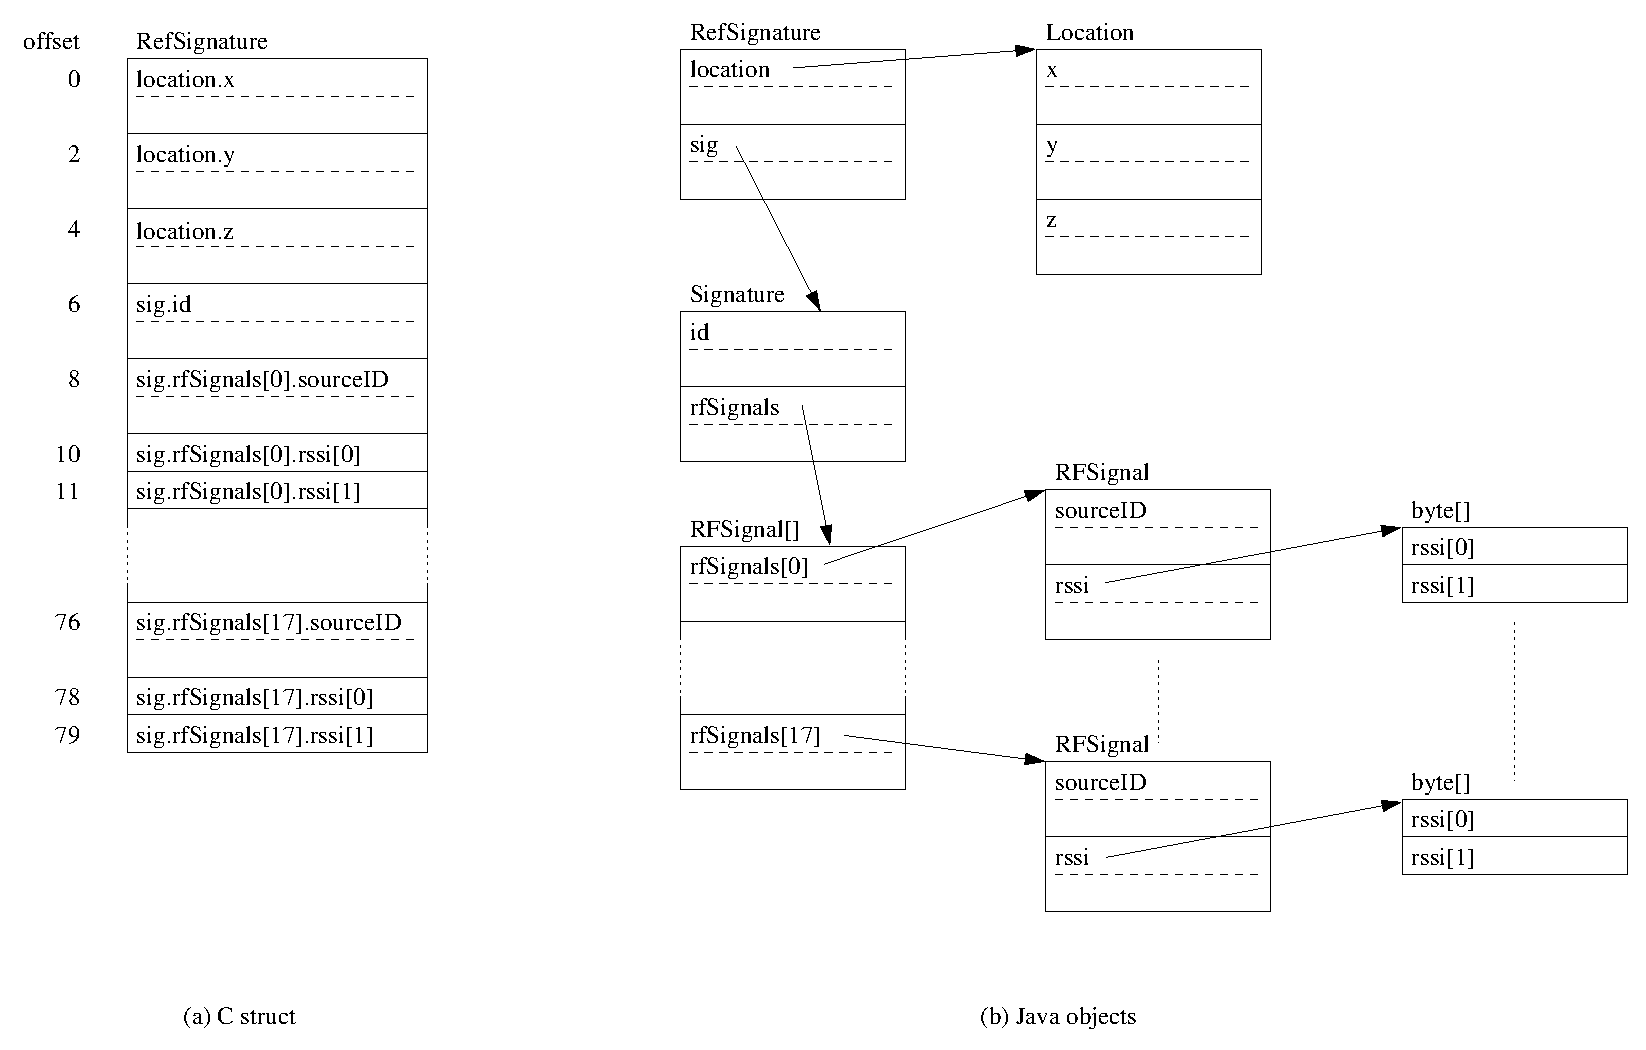
\includegraphics[width=0.9\linewidth]{motetrack-refsignature-objects}
\caption[The \mycode{RefSignature} data structure]{The \mycode{RefSignature} data structure: as a C struct, and as a collection of Java objects}
\label{fig-motetrack-refsignature-objects}
\end{figure}

Since all the arrays are of fixed length, in C the layout of the whole structure is known at compile time, shown in Figure \ref{fig-motetrack-refsignature-objects}. As described in Section \ref{sec-background-jvm-memory}, in Java every object is made up of a list of primitive values: either an int or a reference to another object. In Java we cannot have an array of objects, only an array of \emph{references to} objects. Thus, the most natural way to translate the C structures in Listing \ref{lst-motetrack-data-structure} to Java, is as a collection of objects and arrays on the heap, as shown in the right half of Figure \ref{fig-motetrack-refsignature-objects}. Note that every one of the 18 \mycode{RFSignal} structs becomes an object, which in turn has a pointer to an array of RSSI values.

There are two problems with this. First, since the location of these Java objects is not known until run time, there is a performance penalty for having to follow the chain of references. \mybench{MoteTrack} will loop over the signals in the \mycode{rfSignals} array. Starting from this array, Java needs to do 3 lookups to get to the right RSSI value: the address of the current \mycode{RFSignal} object, the address of the \mycode{rssi} array, and then the actual RSSI value. For the C version, all the offsets are known at compile time, so the compiler can generate a much more efficient loop, directly reading from the right locations.

The second problem is the added memory usage. The C struct only takes up 80 bytes, all used to store data. The Java version allocates a total of 40 objects, 36 of which are spent on the \mycode{RFSignal} objects and their arrays of RSSI values. Each of these requires a heap header, which takes up 5 bytes. In addition, the 18 byte arrays have a 3 byte header, the signal array a 4 byte header, and the whole structure contains a total of 39 references which each take up 2 bytes. In total, the collection of Java objects use $80 + 40*5 + 18*3 + 4 + 39*2 = 416$ bytes.

Combined with \mybench{MoteTrack}'s other data structures, this is too large to fit in memory, which forced us to refactor the 2 element \mycode{rssi} array into two byte variables stored directly in \mycode{RFSignal}, as explained in Section \ref{sec-evaluation-benchmark-implementation-motetrack}. This allowed us to run the benchmark, but a RefSignature still takes up 236 bytes, and reading an RSSI value still takes two lookups instead of one.

Table \ref{tbl-quantitative-results} shows the size of the main data structures used by each benchmark. For most benchmarks that operate on a handful of objects and arrays, the overhead is limited to at most tens of bytes. Besides \emph{MoteTrack}, the \emph{CoreMark} benchmark also has a significant overhead. Here the cause is the linked list of \mycode{ListHead} and \mycode{ListData} objects, each of which has a 5 byte header.

Generally, large arrays of primitive types do not suffer from this problem and can be stored with low relative overhead, but for programmes containing large numbers of small objects the overhead is significant. In some cases this can be mitigated by flattening the structure. Section \ref{sec-evaluation-coremark} described an alternative for \mybench{CoreMark} to replace the linked list with a single array, and in \mybench{MoteTrack}'s case the array of \mycode{RFSignal} objects could be replaced with three separate arrays for \mycode{sourceID}, \mycode{rssi_0} and \mycode{rssi_1}. In both cases the reduced memory overhead comes at a significant cost in readability.




\section{Better language support for shorts and bytes}
\label{sec-small-datatypes}
Because RAM is scarce, 16-bit short and single byte data types are commonly used in sensor node code. The standard JVM only has 32 and 64-bit operations, and variables and stack values are stored as 32-bit, even if the actual type is shorter. On a sensor node this wastes memory, and causes a performance overhead since most nodes have 8-bit or 16-bit architectures. Therefore, many sensor node JVMs, including Darjeeling, introduce 16-bit operations and store values in 16-bit slots.

However, this is only one half of the solution. At the language level, Java defines that an expression evaluates to 32-bits, or 64-bits if at least one operand is a \mycode{long}. Attempting to store this in a 16-bit variable will result in a `lossy conversion' error at compile time, unless explicitly cast to a \mycode{short}.

As an example, if we have 3 \mycode{short} variables, a, b, and c, and want store the sum of b and c in a, a cast is needed to avoid errors from the Java compiler:

\mycode{a=(short)(b+c);}

Passing literal integer values to a method call treats them as ints, even if they are small enough to fit in a smaller type, which results in calls like: 

\mycode{f((byte)1);}

While seemingly a small annoyance, in more complex code that frequently uses of shorts and bytes, these casts can make the code much harder to read. Table \ref{tbl-quantitative-results} shows that over 25 casts per 100 lines of code appear in some benchmarks.

\paragraph{Possible solutions}
%If we want to have an efficient sensor node VM, both from a performance and memory usage perspective, better support for data types smaller than 32-bit integers is necessary.

We argue that C-style automatic narrowing conversions would make most sensor node code more readable, but to leave the option of Java's default behaviour open, this may be implemented as new data types: declaring variable \mycode{a} as \mycode{unchecked short} would implicitly narrow to short when needed, so \mycode{a=b+c;} would not need an explicit cast, while it would if \mycode{a} is declared as a normal \mycode{short}.




\section{Simple type definitions}
\label{sec-typedef}
When developing code for a sensor node, the limited resources often result design patterns different from desktop software. In normal Java code we usually rely on objects for type safety and keeping code readable and easy to maintain. On sensor nodes, objects are expensive and we frequently make use of shorts and ints for a multitude of different tasks for which we would traditionally use objects.

In these situations we often found that our code would be much easier to maintain if there was a way to name new integer types to explicitly indicate their meaning, instead of using many of \mycode{int} or \mycode{short} variables. Having type checking on these types would add a welcome layer of safety.

\paragraph{Possible solutions}
At a minimum, there should be a way to define simple aliases for primitive types, similar to C's \mycode{typedef}. A more advanced option that fits more naturally with Java, would be to have a strict \mycode{typedef} which also does type checking, so that a value of one user defined integer type cannot be accidentally assigned to a variable of another type, without an explicit cast.




\section{Explicit and efficient inlining}
\label{sec-inlining}
Java method calls are inherently more expensive than C functions. On the desktop, JIT compilers can remove much of this overhead, but a sensor node does not have the resources for this. We often found this to be a problem for small helper functions that are frequently called. As an example, the C version of the \mybench{XXTEA} benchmark contains this macro: 

\begin{minted}{c}
    #define MX (((z>>5^y<<2) + (y>>3^z<<4)) \\
                 ^ ((sum^y) + (key[(p&3)^e] ^ z)))
\end{minted}

This macro is called in four places, and implementing it as a lightweight method still slows down the benchmark by 57\%. Tools like ProGuard \cite{proguard} can be used to inline small methods or methods that are only called from a single location, but \mycode{MX} is called from multiple places and is larger than ProGuard's size threshold. This leaves developers with two unattractive options: either leaving it as a method and accepting the performance penalty, or manually copy-pasting the code, which is error-prone and leads to code that is harder to maintain.

Inlining larger methods called from multiple locations does run the risk of increasing code size. However, the data in Table \ref{tbl-quantitative-results} shows the increase in code size is often modest. In two cases the inlined version is actually smaller. The code generated by the AOT compiler for a lightweight method call is still larger than for most other bytecode instructions, and in \emph{CoreMark}'s case inlining the \mycode{ee_isdigit} method means the code directly branches on the result of the inlined expression, instead of having to perform an additional branch on the returned boolean value.

\paragraph{Possible solutions}
Developers should be given more control over inlining, which could be achieved by an \mycode{inline} keyword to force the compiler to inline important methods.



\section{An optimising compiler}
\label{sec-optimising-javac}
As discussed in previous chapters, but listed here again for completeness, Java compilers typically do not optimise the bytecode but translate the source almost as-is. Without a clear performance model it is not always clear which option is faster, and the bytecode is expected to be run by a JIT compiler, which can make better optimisation decisions knowing the target platform and run-time behaviour. However, a sensor node does not have the resources for this and must execute the code as it is received. This leads to significant overhead, for example by repeatedly re-evaluating a constant expression in a loop.

\paragraph{Possible solutions}
Even without a clear performance model, some basic optimisations can be done. Table \ref{tbl-quantitative-results} shows the resulting performance without the manual optimisations discussed in Section \ref{sec-optimisations-manual-java-source-optimisation}. These optimisations could be further expanded, and combining the tasks of the optimiser and infuser can further improve performance as shown in Section \ref{sec-evaluation-other-platforms-word-size}.




\section{Allocating objects on stack}
\label{sec-no-gc}
In Java anything larger than a primitive value has to be allocated on the heap. This introduces a performance overhead, both for allocating the objects, and the occasional run of the garbage collector that may take several thousand cycles.

In our benchmarks we encountered a number of situations where a temporary object was needed. For example, the \mycode{encode} function in the \mybench{LEC} benchmark needs to return two values: \emph{bsi} and the number of bits in \emph{bsi}. In C this is done by passing two pointers to \mycode{encode}. In Java we can wrap both values in a class and either create and return an object from \mycode{encode}, or let the caller create it and pass it as a parameter for \mycode{encode} to fill in.

In code that frequently needs short-lived objects the overhead for allocating them can be significant, and unpredictable garbage collector runs are a problem for code with specific timing constraints. Besides \mybench{LEC}, we saw similar situations in the \mybench{CoreMark} and \mybench{MoteTrack} benchmarks. The problem is especially serious on a sensor node, where the limited amount of memory means the garbage collector is triggered frequently even if relatively few temporary objects are created.

\begin{listing}
\begin{minted}{java}
    public static short LEC(short[] numbers, Stream stream) {
        BSI bsi = new BSI();      // Allocate bsi only once
        for (...) {
            ...
            compress(ri, ri_1, stream, bsi);
            ...
        }
    }

    private static void compress(short ri, short ri_1, Stream stream, BSI bsi) {
        ...
        encode(di, bsi);          // Pass bsi to encode to return both value and length
        ...
    }

    private static void encode(short di, BSI bsi) {
        ...
        bsi.value = ...           // return value and length by setting object fields
        bsi.length = ...
    }
\end{minted}
\caption{Avoiding multiple object allocations in the LEC benchmark}
\label{lst-lec-avoiding-object-allocations}
\end{listing}

This overhead can often be reduced by allocating objects earlier and reusing the same objects in a loop. In Listing \ref{lst-lec-avoiding-object-allocations} this is implemented for the \mybench{LEC} benchmark, where the \mycode{bsi} object is used to return two values from \mycode{encode} to \mycode{compress}. Instead of creating a new object in each iteration in the \mycode{compress} method where it is needed, \mycode{bsi} is created once, outside of the main loop, and passed to \mycode{compress} multiple times.

This technique of pulling object creation up the call chain can often be used to remove this sort of overhead, and it worked in all three benchmarks mentioned before. However, it gets very cumbersome if the number of objects is more than one or two, or if they need to be passed through multiple layers. Readability is also reduced, since objects that are only needed in a specific location are now visible from a much larger scope. Table \ref{tbl-quantitative-results} shows the performance without this optimisation.

\paragraph{Possible solutions}
On desktop JVMs, escape analysis \cite{Choi:1999uw, Goetz:2005uy} is used to determine if an object can be safely allocated on the stack instead of the heap, thus saving both the cost of heap allocation, and the occasional garbage collection run triggered by it.

While the analysis of the bytecode required for this is far too complex for a sensor node, it could be done offline, similar to TakaTuka's offline garbage collector analysis \cite{Aslam:2011thesis}. The bytecode can then be extended by adding special versions of the \mycode{new} opcodes to instruct the VM to place an object in the stack frame instead of on the heap. A field should also be added to the method header to tell the VM how much extra space for stack objects needs to be reserved in the stack frame.

There is a risk to doing this automatically. In CapeVM, the split between heap and stack memory is fixed, and both are limited. If the compiler automatically puts all objects that could be on the stack in the stack frame instead of on the heap, we may end up with an empty heap, and a stack overflow. Therefore, it is better to leave this optimisation to the developer by also introducing a new keyword at the language level, so developers can explicitly indicate which objects go on the stack and which on the heap. Of course escape analysis is still necessary to check at compile time that this keyword is only used in places where it is legal for the object to be allocated on the stack.




\section{Reconsidering advanced language features}
\label{sec-advanced-features}
Finally, we conclude with some discussion on more fundamental language design choices. Many sensor node JVMs implement some of Java's more advanced features, but we are not convinced this is always a good choice on a sensor node.

While features like threads, exceptions and garbage collection are all useful, they come at a cost. The trade-off for a sensor node VM is significantly different from a desktop VM: many of Java's more advanced features are vital to large-scale software development, but the size of sensor nodes programmes is much smaller. And while VM size is not an issue on the desktop, these features are relatively expensive to implement on a sensor node with limited flash memory. We believe a VM developed from scratch, with the aim of providing platform independence, safety, and performance through AOT compilation, would end up with a design very different from the JVM.

Table \ref{tab-vm-size} shows the code size in Darjeeling for some features discussed below. This was determined by only counting the size of functions directly related to specific features. The actual cost is higher since some, especially garbage collection, also add complexity to other functions throughout the VM. Combined, the features below and the string functions mentioned in Section \ref{sec-std-lib} make up about half of the original Darjeeling VM.

Besides an increase in VM size, these features also cause a performance penalty, and features such as threads and exceptions are much harder to implement in an AOT compiler where we cannot implement them in the interpreter loop. This means that if we care about performance and the corresponding reduction in CPU energy consumption, we either have to give them up, or spend considerably more in terms of VM complexity and size.


\subsection{Threads}
As shown in Table \ref{tab-vm-size}, support for threads accounts for about 10\% of the VM size, if we exclude the string library. In addition, each thread requires a stack. If the VM allocates a fixed block, it must be large enough to avoid stack overflows, but too large a block wastes precious RAM. Darjeeling allocates each stack as a linked list of frames on the heap. This is memory efficient, but allocating on the heap is slower and will occasionally trigger the garbage collector.

A more cooperative concurrency model, where lightweight tasks voluntarily yield the CPU and share a single stack, is more appropriate for sensor nodes. This is also the approach to concurrency chosen by a number of native code systems, including \emph{t-kernel} \cite{Gu:2005un}, nesC \cite{Gay:2003up}, and more recently Amulet \cite{Hester:2016je}.


\subsection{Exceptions}
In terms of code size, exceptions are not very expensive to implement in an interpreter, but they are hard to implement in an AOT compiler. We also feel the advantage of having exceptions is much lower than the other features mentioned in this section, since they could be easily replaced with return values to signal errors.


\subsection{Virtual methods}
It is hard to quantify the overhead of implementing virtual methods since the code for handling them is integrated into several functions. In terms of size it is likely less than 2 KB, but the performance overhead is considerable. The target of a virtual method call must be resolved at run time, they cannot be made lightweight, and an AOT compiler can generate much more efficient code for calls to static methods.

In practice we seldom use virtual methods in sensor node code, but some form of indirect calls is necessary for things like signal handling. It should be possible to develop a more lightweight form of function pointers that can be implemented efficiently. However, the details will require more careful study.


\subsection{Garbage collection}
Finally, garbage collection is clearly the most intrusive aspect of the JVM to change. While the first three features could be changed with minor modifications to Java, the managed heap is at its very core.

Still, there are good reasons for considering alternatives. Table \ref{tab-vm-size} shows the garbage collector functions in Darjeeling add up to about 3.5 KB, but the actual cost is much higher as many other parts of Darjeeling are influenced by the garbage collector.

Specifically, it is the reason Darjeeling splits references and integers throughout the VM. This makes it easy for the garbage collector to find live references, but leads to significant code duplication and complexity. Using AOT compilation, the split stack adds overhead to maintain this state, and requires two extra registers as a second stack pointer that cannot be used for stack caching.




\section{Building better sensor node VMs}
In this chapter we described a number of issues we encountered over the years while using and developing sensor node VMs. They may not apply to every scenario, but the wide range of the issues presented here, and the data in Table \ref{tbl-quantitative-results}, suggest many applications will be affected by at least some.

Most sensor node VMs already modify the instruction set of the original VM and usually support only a subset of the original language. The issues described here indicate these changes do not go far enough, and we still need to refine our VMs further to make them truly useful in real-world projects.

There are two possible paths to follow: a number of issues can be solved by improving existing Java-based VMs. Staying close to Java has the advantage of being able to reuse existing knowledge and infrastructure.

However some of the issues require more invasive changes to both the source language and VM. If the goal is to run platform independent code safely and efficiently, rather than running Java, we should start from the specific requirements and constraints of sensor node software development, which would lead to more lightweight features and a more predictable memory model.

For either path, we hope the points presented in this chapter can help in the development of better future sensor node VMs.
